\documentclass[a4paper,11pt]{article}
\usepackage[margin=2.2cm]{geometry}
\usepackage{amsmath,amssymb,xcolor}
\usepackage{tikz,pgfplots}
\usetikzlibrary{positioning,arrows.meta,calc,fit,backgrounds,automata}
\pgfplotsset{compat=1.17}
% ---------------------------------------------------------------
% Shared TikZ styles. Fonts are inherited from the host document,
% so labels match the body text automatically (no hard-coded fonts).
% Required: \usepackage{tikz,pgfplots}, \usetikzlibrary{positioning,
%   arrows.meta,calc,fit,backgrounds,automata,shapes.geometric}
% ---------------------------------------------------------------
\definecolor{oiBlue}{HTML}{0072B2}
\definecolor{oiOrange}{HTML}{E69F00}
\definecolor{oiGreen}{HTML}{009E73}
\definecolor{oiVerm}{HTML}{D55E00}
\definecolor{oiSky}{HTML}{56B4E9}

\tikzset{
  >={Stealth[length=1.6mm]},
  every node/.append style={font=\footnotesize},
  block/.style={draw, rounded corners=1pt, minimum width=22mm, minimum height=6.5mm,
                align=center, line width=0.5pt, inner sep=2pt},
  attn/.style={block, fill=oiBlue!15, draw=oiBlue!80!black},
  ffn/.style={block, fill=oiGreen!15, draw=oiGreen!60!black},
  norm/.style={block, fill=oiOrange!18, draw=oiOrange!70!black, minimum height=5mm},
  embed/.style={block, fill=oiSky!20, draw=oiSky!60!black},
  head/.style={block, fill=oiVerm!12, draw=oiVerm!70!black},
  flow/.style={->, line width=0.5pt},
  skip/.style={->, line width=0.5pt, dashed, oiVerm!80!black},
  sum/.style={circle, draw, inner sep=0.8pt, line width=0.5pt},
  state/.style={circle, draw, minimum size=9mm, line width=0.5pt, inner sep=1pt},
  accepting/.style={double, double distance=1pt},
}

\usepackage{caption}
\usepackage{hyperref}
\begin{document}
\section*{Native TikZ \& PGFPlots showcase}
All figures below are pure vector graphics; labels inherit the document font.
\begin{figure}[h]\centering% Transformer encoder block stack (Vaswani et al. style), fully native TikZ.
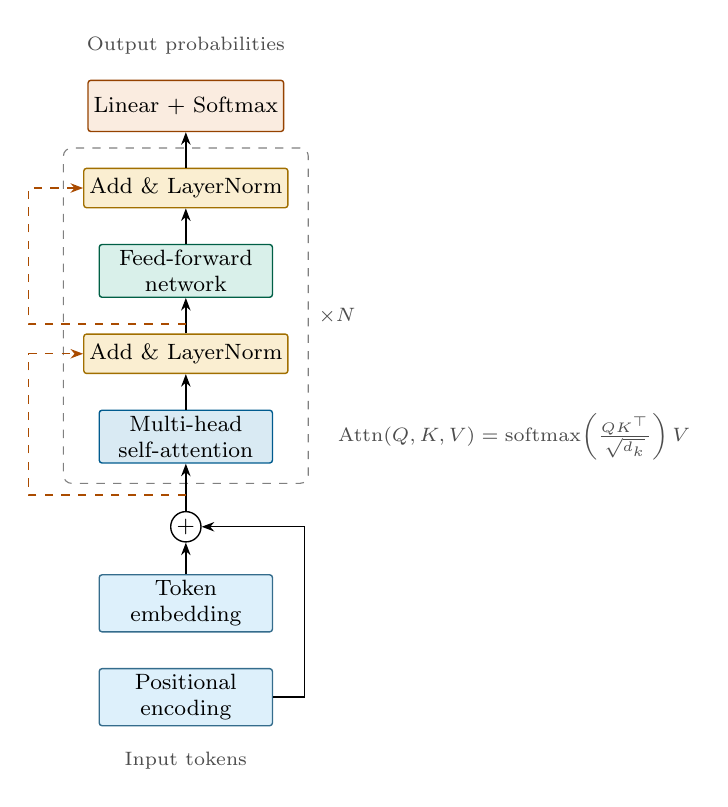
\begin{tikzpicture}[node distance=4.5mm and 6mm]
  % --- input path
  \node[embed] (tok) {Token\\embedding};
  \node[embed, below=of tok] (pos) {Positional\\encoding};
  \node[sum, above=4mm of tok] (add0) {$+$};
  \draw[flow] (tok) -- (add0);
  \draw[flow] (pos.east) -- ++(4mm,0) |- (add0.east);
  % --- encoder layer (repeated N times)
  \node[attn, above=6mm of add0] (mha) {Multi-head\\self-attention};
  \node[norm, above=of mha] (n1) {Add \& LayerNorm};
  \node[ffn, above=of n1] (ff) {Feed-forward\\network};
  \node[norm, above=of ff] (n2) {Add \& LayerNorm};
  \node[head, above=of n2] (out) {Linear + Softmax};
  \draw[flow] (add0) -- (mha);
  \draw[flow] (mha) -- (n1);
  \draw[flow] (n1) -- (ff);
  \draw[flow] (ff) -- (n2);
  \draw[flow] (n2) -- (out);
  % --- residual (skip) connections
  \draw[skip] ($(add0.north)+(0,2mm)$) -- ++(-20mm,0) |- (n1.west);
  \draw[skip] ($(n1.north)+(0,1.2mm)$) -- ++(-20mm,0) |- (n2.west);
  % --- repeat bracket
  \begin{scope}[on background layer]
    \node[draw=black!50, dashed, rounded corners=3pt, inner sep=2.5mm,
          fit=(mha)(n1)(ff)(n2), label={[font=\scriptsize, black!70]right:$\times N$}] {};
  \end{scope}
  % --- annotations
  \node[right=7mm of mha, font=\scriptsize, align=left, text=black!70]
        {$\mathrm{Attn}(Q,K,V)=\mathrm{softmax}\!\left(\frac{QK^{\top}}{\sqrt{d_k}}\right)V$};
  \node[above=2mm of out, font=\scriptsize, text=black!70] {Output probabilities};
  \node[below=2mm of pos, font=\scriptsize, text=black!70] {Input tokens};
\end{tikzpicture}
\caption{Transformer encoder stack with residual connections (TikZ).}\end{figure}
\begin{figure}[h]\centering% Finite-state vending controller. Transition labels are placed explicitly
% so the diamond layout remains readable at journal-page scale.
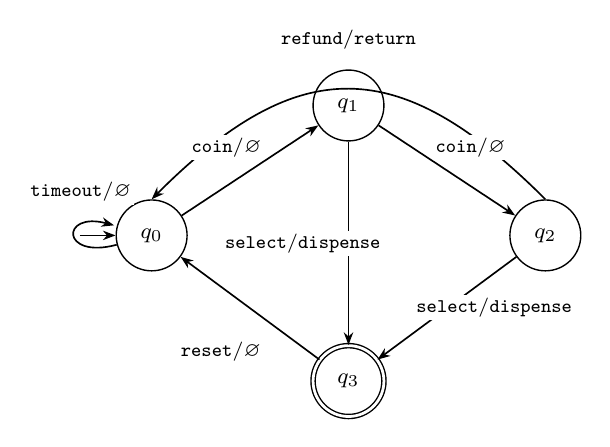
\begin{tikzpicture}[semithick]
  \node[state, initial, initial text=] (s0) at (0,0) {$q_0$};
  \node[state] (s1) at (2.5,1.65) {$q_1$};
  \node[state] (s2) at (5,0) {$q_2$};
  \node[state, accepting] (s3) at (2.5,-1.85) {$q_3$};

  % Transitions
  \path[->]
    (s0) edge[loop left] (s0)
    (s0) edge (s1)
    (s1) edge (s2)
    (s1) edge (s3)
    (s2) edge (s3)
    (s3) edge (s0);
  \draw[->] (s2.north) to[out=135,in=45,looseness=1.35] (s0.north);

  % Explicit labels avoid collisions between converging transitions.
  \node[font=\scriptsize, fill=white, inner sep=1pt] at (-0.9,0.55) {$\mathtt{timeout}/\varnothing$};
  \node[font=\scriptsize, fill=white, inner sep=1pt] at (0.95,1.12) {$\mathtt{coin}/\varnothing$};
  \node[font=\scriptsize, fill=white, inner sep=1pt] at (4.05,1.12) {$\mathtt{coin}/\varnothing$};
  \node[font=\scriptsize, fill=white, inner sep=1pt] at (1.92,-0.10) {$\mathtt{select}/\mathtt{dispense}$};
  \node[font=\scriptsize, fill=white, inner sep=1pt] at (4.35,-0.92) {$\mathtt{select}/\mathtt{dispense}$};
  \node[font=\scriptsize, fill=white, inner sep=1pt] at (0.88,-1.48) {$\mathtt{reset}/\varnothing$};
  \node[font=\scriptsize, fill=white, inner sep=1pt] at (2.5,2.48) {$\mathtt{refund}/\mathtt{return}$};
\end{tikzpicture}
\caption{Finite state machine with Mealy-style transitions (TikZ \texttt{automata}).}\end{figure}
\begin{figure}[h]\centering% Closed-loop feedback control system with PID controller, plant and sensor.
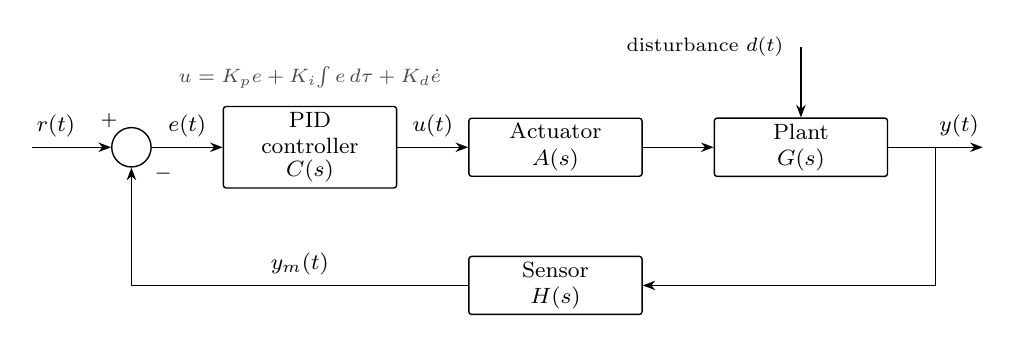
\begin{tikzpicture}[node distance=9mm and 9mm, auto]
  \node[coordinate] (in) {};
  \node[sum, minimum size=5mm, right=10mm of in] (cmp) {};
  \node[block, right=of cmp] (pid) {PID\\controller\\[-1pt]$C(s)$};
  \node[block, right=of pid] (act) {Actuator\\$A(s)$};
  \node[block, right=of act] (plant) {Plant\\$G(s)$};
  \node[coordinate, right=12mm of plant] (out) {};
  \node[block, below=10mm of act] (sens) {Sensor\\$H(s)$};
  \node[coordinate, above=9mm of plant] (dist) {};
  \draw[flow] (in) -- node[pos=0.3] {$r(t)$} (cmp);
  \draw[flow] (cmp) -- node {$e(t)$} (pid);
  \draw[flow] (pid) -- node {$u(t)$} (act);
  \draw[flow] (act) -- (plant);
  \draw[flow] (plant) -- node[pos=0.75] {$y(t)$} (out);
  \draw[flow] ($(plant.east)+(6mm,0)$) |- (sens.east);
  \draw[flow] (sens.west) -| node[pos=0.25, swap] {$y_m(t)$} (cmp.south);
  \draw[flow] (dist) -- (plant.north);
  \node[left=1mm of dist, font=\scriptsize] {disturbance $d(t)$};
  \node[font=\scriptsize] at ($(cmp.north west)+(-1mm,1.5mm)$) {$+$};
  \node[font=\scriptsize] at ($(cmp.south east)+(2.2mm,-1.5mm)$) {$-$};
  \node[above=1mm of pid, font=\scriptsize, text=black!70, align=center]
       {$u=K_p e+K_i\!\int e\,d\tau+K_d\dot e$};
\end{tikzpicture}
\caption{Closed-loop PID control system (TikZ, \texttt{positioning}).}\end{figure}
\begin{figure}[h]\centering\begin{minipage}{0.7\linewidth}% Step response of a second-order system for several damping ratios,
% plotted natively with PGFPlots (vector, fonts match the document).
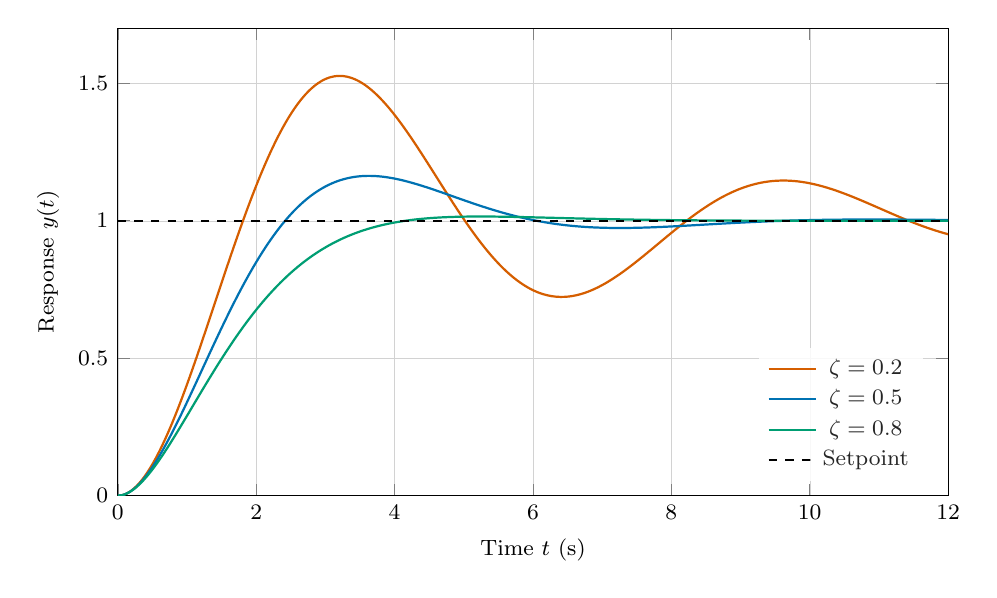
\begin{tikzpicture}
  \begin{axis}[
      width=\linewidth, height=0.62\linewidth,
      xlabel={Time $t$ (s)}, ylabel={Response $y(t)$},
      xmin=0, xmax=12, ymin=0, ymax=1.7,
      grid=both, grid style={line width=.1pt, draw=gray!20}, major grid style={draw=gray!35},
      legend pos=south east, legend style={font=\scriptsize, draw=none, fill=white, fill opacity=0.85},
      every axis plot/.append style={line width=0.8pt}, samples=200, smooth, domain=0:12,
      tick label style={font=\footnotesize}, label style={font=\footnotesize}]
    \def\wn{1}
    \addplot[oiVerm]{1 - exp(-0.2*\wn*x)*(cos(deg(\wn*sqrt(1-0.04)*x)) + (0.2/sqrt(1-0.04))*sin(deg(\wn*sqrt(1-0.04)*x)))};
    \addlegendentry{$\zeta=0.2$}
    \addplot[oiBlue]{1 - exp(-0.5*\wn*x)*(cos(deg(\wn*sqrt(1-0.25)*x)) + (0.5/sqrt(1-0.25))*sin(deg(\wn*sqrt(1-0.25)*x)))};
    \addlegendentry{$\zeta=0.5$}
    \addplot[oiGreen]{1 - exp(-0.8*\wn*x)*(cos(deg(\wn*sqrt(1-0.64)*x)) + (0.8/sqrt(1-0.64))*sin(deg(\wn*sqrt(1-0.64)*x)))};
    \addlegendentry{$\zeta=0.8$}
    \addplot[black, dashed, domain=0:12, samples=2]{1};
    \addlegendentry{Setpoint}
  \end{axis}
\end{tikzpicture}
\end{minipage}\caption{Second-order step responses (PGFPlots).}\end{figure}
\end{document}
